\chapter{Resultados}
\label{sec:Resultados}

Este capítulo irá mostrar os resultados obtidos através dos dados colhidos durante os ensaios de envelhecimento detalhados na seção \ref{sec:MetEnsaios}. Serão apresentados os valores iniciais e finais das frequências dos osciladores, as curvas de como as frequências variaram com o tempo de exposição ao calor, as curvas frequência por temperatura para diferentes tempos de exposição e as curvas das medidas durante o relaxamento dos dispositivos.

\section{Medidas Iniciais}
\label{sec:ResMedidasIniciais}

As primeiras medidas foram realizadas em temperatura ambiente antes dos ensaios iniciarem, para se ter as frequências iniciais dos osciladores. A Tabela \ref{tab:FreqIniciais} mostra esses valores os dois osciladores de cada placa. Esses valores serão utilizados como valor unitário quando os valores das frequências medidas estiverem normalizado.

\begin{table}[H]
\centering
\caption{Frequências iniciais dos osciladores.}
\begin{tabular}{l|cc|cc|}
\cline{2-5}
 & \multicolumn{2}{c|}{\textbf{Altera DE2}} & \multicolumn{2}{c|}{\textbf{ZedBoard}} \\ \cline{2-5} 
 & \multicolumn{1}{c|}{\textbf{1001}} & \textbf{4999} & \multicolumn{1}{c|}{\textbf{1001}} & \textbf{4999} \\ \hline
\multicolumn{1}{|l|}{\textbf{Estressados}} & \multicolumn{1}{c|}{1805kHz} & 364,9kHz & \multicolumn{1}{c|}{1470kHz} & 276,5kHz \\ \hline
\multicolumn{1}{|l|}{\textbf{Não Estressados}} & \multicolumn{1}{c|}{1756kHz} & 354,5kHz & \multicolumn{1}{c|}{1520kHz} & 286kHz \\ \hline
\end{tabular}
\label{tab:FreqIniciais}
\end{table}
\section{Comparação das Curvas à temperatura ambiente}
\label{sec:ResTAmb}

As medidas em temperatura ambiente foram realizadas no início de cada um dos ciclos de estresse (como indicado na Tabela \ref{tab:TempoDia}) antes de ligar a câmara térmica. As medidas apresentam uma certa oscilação devido a variabilidade da temperatura ambiente.

A Figura \ref{fig:TAmbEstressadas} mostra as curvas das frequências normalizadas dos osciladores das placas que foram estressadas em relação ao tempo de exposição. Nela é possível ver um comportamento da DE2 de uma diminuição da frequência no inicio dos ensaios seguido de uma estabilidade. Já a ZedBoard apresentou uma degradação maior e ao longo de todas as medidas, o formato da curva é o esperado segundo a Equação \ref{eq:VthTempo} que indica uma degradação decrescente.

\begin{figure}[H]
    \centering
    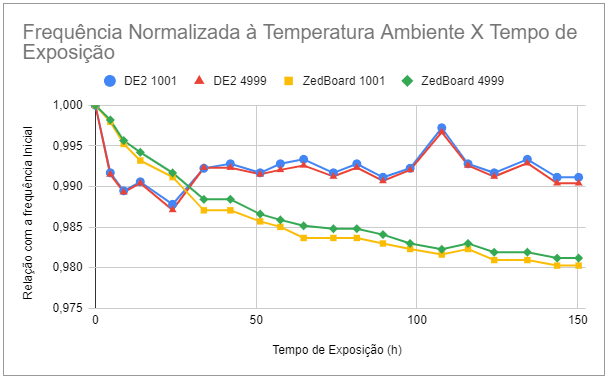
\includegraphics[scale=0.75]{figures/Resultados/TAmbEstressadas}
    \caption{Comparação das duas placas à temperatura ambiente. Fonte: O Autor}
    \label{fig:TAmbEstressadas}
\end{figure}

A Figura \ref{fig:TAmbDE2} mostra as curvas das frequências normalizadas dos osciladores das placas  DE2, tanto a que foi estressada termicamente quanto a que não foi estressada, em relação ao tempo de exposição.

É possível observar que a placa que não foi estressada apresenta uma curva semelhante à que foi estressada, o que pode indicar que o FPGA da DE2 não sofreu do NBTI e que a degradação é apenas decorrente do uso prolongado da placa ou que a temperatura não foi um fator tão relevante para o fenômeno, tendo sido, ambas as placas, afetados por ele da mesma forma.

\begin{figure}[H]
    \centering
    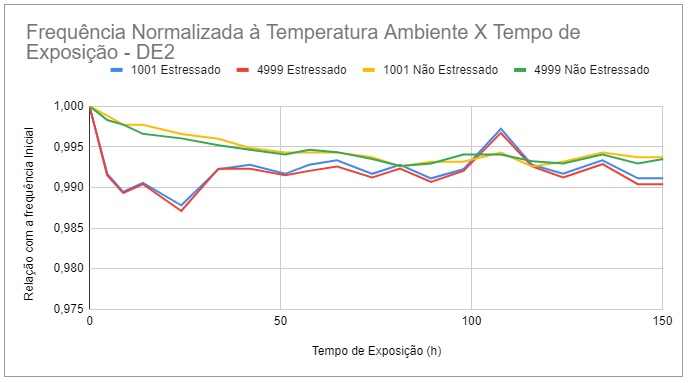
\includegraphics[scale=0.75]{figures/Resultados/TAmbDE2}
    \caption{Curva das placas DE2 à temperatura ambiente. Fonte: O Autor}
    \label{fig:TAmbDE2}
\end{figure}

As mesmas curvas são mostradas na Figura \ref{fig:TAmbZedBoard}, porém para as placas ZedBoard. Diferentemente da DE2, para a ZedBoard o comportamento entre a placa que foi estressada e a que não foi apresentaram uma diferença considerável, ambas possuem o mesmo formato porém a estressada demonstra uma queda maior na frequência.

\begin{figure}[H]
    \centering
    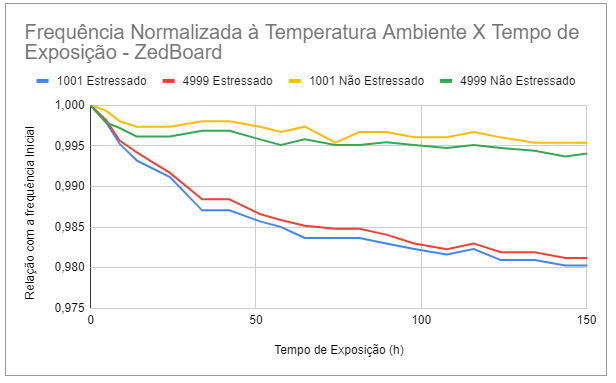
\includegraphics[scale=0.75]{figures/Resultados/TAmbZedBoard}
    \caption{Curva das placas DE2 a temperatura ambiente. Fonte: O Autor}
    \label{fig:TAmbZedBoard}
\end{figure}

A Tabela \ref{tab:FreqFinaisTAmb} mostra os valores finais das frequências de cada um dos osciladores. Já a Tabela \ref{tab:DegradFinaisTAmb} mostra a porcentagem da degradação das frequências em relação às frequências iniciais.

\begin{table}[H]
\centering
\caption{Frequências finais dos osciladores à temperatura ambiente.}
\begin{tabular}{l|cccc|}
\cline{2-5}
 & \multicolumn{4}{c|}{\textbf{Frequência (kHz)}} \\ \cline{2-5} 
 & \multicolumn{2}{c|}{\textbf{Altera DE2}} & \multicolumn{2}{c|}{\textbf{ZedBoard}} \\ \cline{2-5} 
 & \multicolumn{1}{c|}{\textbf{1001}} & \multicolumn{1}{c|}{\textbf{4999}} & \multicolumn{1}{c|}{\textbf{1001}} & \textbf{4999} \\ \hline
\multicolumn{1}{|l|}{\textbf{Estressados}} & \multicolumn{1}{c|}{1789} & \multicolumn{1}{c|}{361,4} & \multicolumn{1}{c|}{1441} & 271,3 \\ \hline
\multicolumn{1}{|l|}{\textbf{Não Estressados}} & \multicolumn{1}{c|}{1745} & \multicolumn{1}{c|}{352,2} & \multicolumn{1}{c|}{1513} & 284,3 \\ \hline
\end{tabular}
\label{tab:FreqFinaisTAmb}
\end{table}

\begin{table}[H]
\centering
\caption{Degradação na frequência dos osciladores à temperatura ambiente.}
\begin{tabular}{l|cr|cr|}
\cline{2-5}
 & \multicolumn{2}{c|}{\textbf{Altera DE2}} & \multicolumn{2}{c|}{\textbf{ZedBoard}} \\ \cline{2-5} 
 & \multicolumn{1}{c|}{\textbf{1001}} & \multicolumn{1}{c|}{\textbf{4999}} & \multicolumn{1}{c|}{\textbf{1001}} & \multicolumn{1}{c|}{\textbf{4999}} \\ \hline
\multicolumn{1}{|l|}{\textbf{Estressados}} & \multicolumn{1}{r|}{0,89\%} & 0,96\% & \multicolumn{1}{r|}{1,97\%} & 1,88\% \\ \hline
\multicolumn{1}{|l|}{\textbf{Não Estressados}} & \multicolumn{1}{r|}{0,63\%} & 0,65\% & \multicolumn{1}{r|}{0,46\%} & 0,59\% \\ \hline
\end{tabular}
\label{tab:DegradFinaisTAmb}
\end{table}

Na Tabela \ref{tab:DegradFinaisTAmb} é confirmado o que foi visto na Figura \ref{fig:TAmbEstressadas} de que a ZedBoard apresentou uma degradação maior que a DE2. Além disso, nela também é visível que a diferença entre o dispositivo estressado e o não estressado é consideravelmente maior no caso da ZedBoard do que no caso da DE2, corroborando com o mostrado nas Figuras \ref{fig:TAmbDE2} e \ref{fig:TAmbZedBoard}.

Um fato que ficou evidente aqui e se repetirá nas seções seguintes é que o comportamento dos osciladores de uma mesma placa, de 1001 e de 4999 inversores, foi semelhante.

Um problema encontrado nestas medidas foi, justamente, a variabilidade da temperatura ambiente, que, por ter influência no valor da frequência, causou um certo ruído nas medidas, principalmente nas da DE2 que foi estressada.
\section{Comparação das Curvas a 135ºC}
\label{sec:ResT135}

Considerando o problema com a variabilidade da temperatura ambiente também foram realizadas medidas na temperatura de 135°C, por ser a temperatura que a câmara térmica estabilizava.

As medidas nessa temperatura só começaram a ser feitas a partir de 14 horas de exposição, pelo fato de nos primeiros ciclos ter sido usado temperaturas mais baixas para verificar se haveriam danos críticos aos dispositivos, como descrito na Seção \ref{sec:MetEnsaios}.

A Figura \ref{fig:T135DE2} mostra as curvas das frequências normalizadas dos osciladores das placas  DE2 que foi estressada termicamente em relação ao tempo de exposição. Nela é visto que a degradação continuou, mesmo que pequena, até o fim dos ensaios, o que não podia ser observado na Figura \ref{fig:TAmbDE2} devido a variação da temperatura ambiente.

\begin{figure}[H]
    \centering
    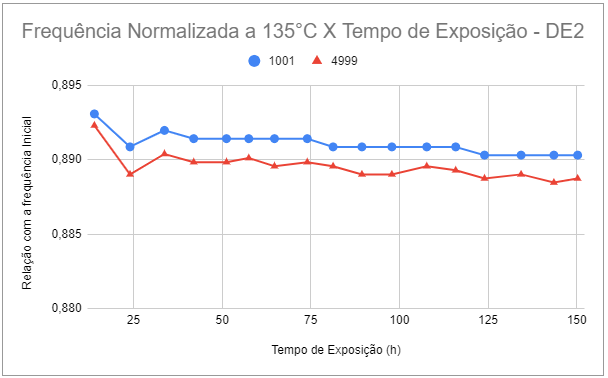
\includegraphics[scale=0.75]{figures/Resultados/T135DE2}
    \caption{Curva da DE2 a 135ºC. Fonte: O Autor}
    \label{fig:T135DE2}
\end{figure}

A Figura \ref{fig:T135ZedBoard} mostra as curvas para a ZedBoard, possuindo um comportamento semelhante ao discutido sobre a Figura \ref{fig:TAmbZedBoard}.

\begin{figure}[H]
    \centering
    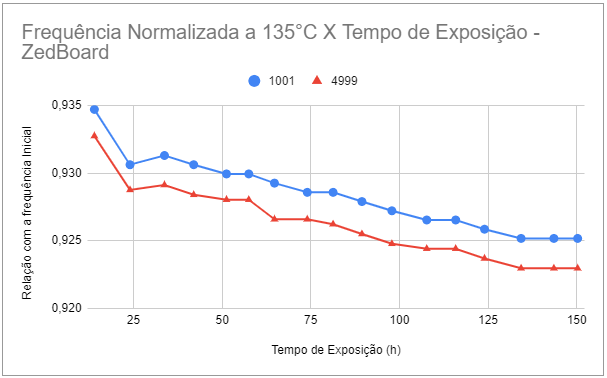
\includegraphics[scale=0.75]{figures/Resultados/T135ZedBoard}
    \caption{Curva da ZedBoard a 135ºC. Fonte: O Autor}
    \label{fig:T135ZedBoard}
\end{figure}

A Figura \ref{fig:T135Ambas} mostras as duas as curvas das Figura \ref{fig:T135DE2} e \ref{fig:T135ZedBoard} juntas no mesmo gráfico.

\begin{figure}[H]
    \centering
    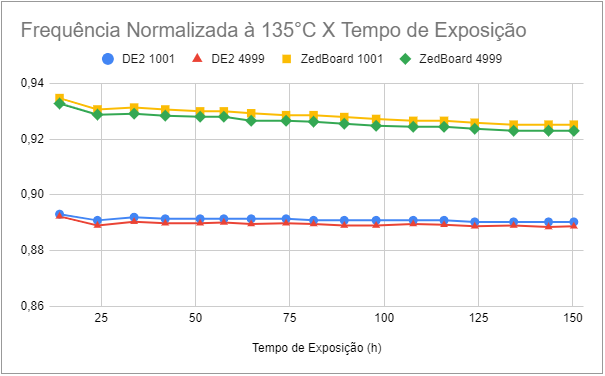
\includegraphics[scale=0.75]{figures/Resultados/T135Ambas}
    \caption{Comparação das duas placas a 135ºC. Fonte: O Autor}
    \label{fig:T135Ambas}
\end{figure}

A Tabela \ref{tab:FreqT135} mostra as frequências iniciais e finais dos osciladores das duas placas que foram estressadas.

\begin{table}[H]
\centering
\caption{Frequências iniciais e finais dos osciladores a 135°C.}
\begin{tabular}{l|cccc|}
\cline{2-5}
 & \multicolumn{4}{c|}{\textbf{Frequência (kHz)}} \\ \cline{2-5} 
 & \multicolumn{2}{c|}{\textbf{Altera DE2}} & \multicolumn{2}{c|}{\textbf{ZedBoard}} \\ \cline{2-5} 
 & \multicolumn{1}{c|}{\textbf{1001}} & \multicolumn{1}{c|}{\textbf{4999}} & \multicolumn{1}{c|}{\textbf{1001}} & \textbf{4999} \\ \hline
\multicolumn{1}{|c|}{\textbf{Inicial}} & \multicolumn{1}{c|}{1612} & \multicolumn{1}{c|}{325,6} & \multicolumn{1}{c|}{1374} & 257,9 \\ \hline
\multicolumn{1}{|c|}{\textbf{Final}} & \multicolumn{1}{c|}{1607} & \multicolumn{1}{c|}{324,3} & \multicolumn{1}{c|}{1360} & 255,2 \\ \hline
\end{tabular}
\label{tab:FreqT135}
\end{table}

\section{Comparação das Curvas Frequência X Temperatura}

\begin{figure}[H]
    \centering
    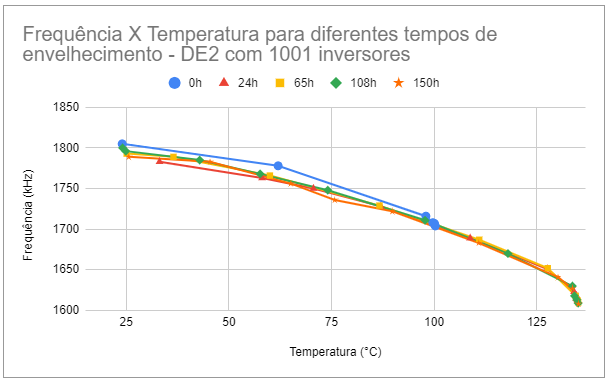
\includegraphics[scale=0.75]{figures/Resultados/FreqXTempDE21001}
    \caption{Curva Freqência por Temperatura do oscilador com 1001 inversores da placa DE2. Fonte: O Autor}
    \label{fig:FreqXTempDE21001}
\end{figure}

\begin{figure}[H]
    \centering
    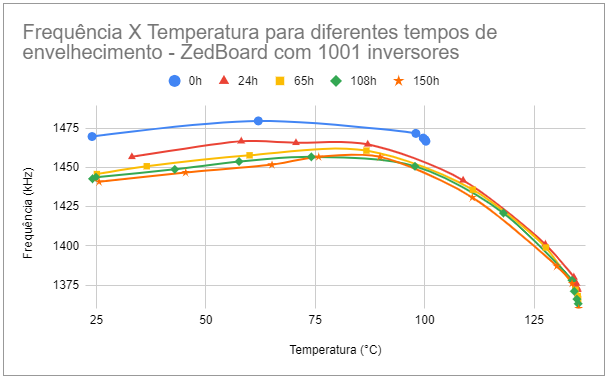
\includegraphics[scale=0.75]{figures/Resultados/FreqXTempZedBoard1001}
    \caption{Curva Freqência por Temperatura do oscilador com 1001 inversores da placa ZedBoard. Fonte: O Autor}
    \label{fig:FreqXTempZedBoard1001}
\end{figure}
\section{Comparação das Curvas de relaxamento}
\label{sec:ResRelax}

Após os ensaios de envelhecimento foram realizadas medidas nos dispositivos para verificar a recuperação da degradação infligida a eles.

A Figura \ref{fig:RelaxEstressadas} mostra as curvas das frequências normalizadas ao longo do tempo de relaxamento das placas que foram estressadas termicamente. Nela se vê que os FPGAs da altera recuperaram mais que os da ZedBoard, e que ele apresenta uma tendência de continuar degradando após o fim dos ensaios, enquanto a ZedBoard apresentou uma estabilização na frequência.

\begin{figure}[H]
    \centering
    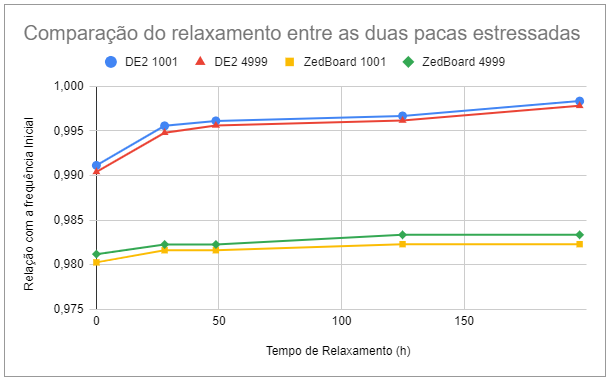
\includegraphics[scale=0.75]{figures/Resultados/RelaxEstressadas}
    \caption{Comparação do relaxamento das duas placas. Fonte: O Autor}
    \label{fig:RelaxEstressadas}
\end{figure}

É demonstrado na Figura \ref{fig:RelaxDE2} como as duas placas DE2 se comportaram ao longo do tempo de relaxamento. É visível que as duas apresentaram semelhança no formato da curva, inclusive alcançando um valor próximo na última medida. 

\begin{figure}[H]
    \centering
    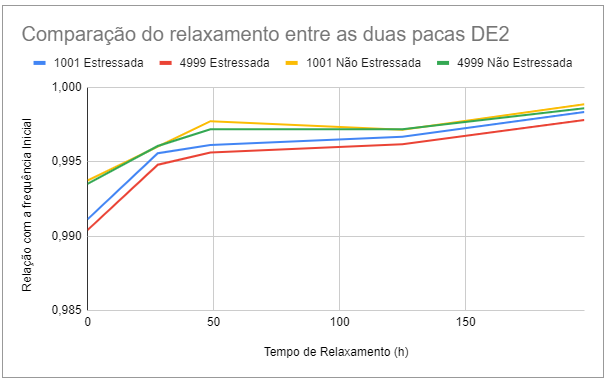
\includegraphics[scale=0.75]{figures/Resultados/RelaxDE2}
    \caption{Curva de relaxamento das placas DE2. Fonte: O Autor}
    \label{fig:RelaxDE2}
\end{figure}

Uma comparação da recuperação das duas ZedBoard é ilustrada na Figura \ref{fig:RelaxZedBoard} onde é possível observar que o formato da curva é semelhante, porém, devido ao valor diferente de degradação que tiveram, a placa estressada recuperou menos proporcionalmente.

\begin{figure}[H]
    \centering
    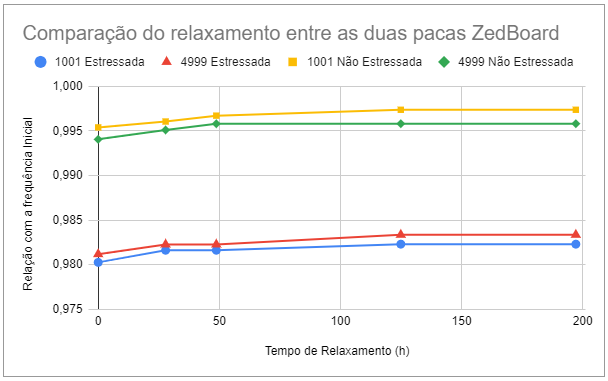
\includegraphics[scale=0.75]{figures/Resultados/RelaxZedBoard}
    \caption{Curva de relaxamento das placas ZedBoard. Fonte: O Autor}
    \label{fig:RelaxZedBoard}
\end{figure}

A Tabela \ref{tab:Relax} mostra o percentual da frequência inicial que foi recuperado durante o período de relaxamento. 

\begin{table}[H]
\centering
\caption{Frequência recuperada.}
\begin{tabular}{l|cccc|}
\cline{2-5}
 & \multicolumn{4}{c|}{\textbf{Recuperação (\%)}} \\ \cline{2-5} 
 & \multicolumn{2}{c|}{\textbf{Altera DE2}} & \multicolumn{2}{c|}{\textbf{ZedBoard}} \\ \cline{2-5} 
 & \multicolumn{1}{c|}{\textbf{1001}} & \multicolumn{1}{c|}{\textbf{4999}} & \multicolumn{1}{c|}{\textbf{1001}} & \textbf{4999} \\ \hline
\multicolumn{1}{|l|}{\textbf{Estressados}} & \multicolumn{1}{c|}{0,72} & \multicolumn{1}{c|}{0,74} & \multicolumn{1}{c|}{0,20} & 0,22 \\ \hline
\multicolumn{1}{|l|}{\textbf{Não Estressados}} & \multicolumn{1}{c|}{0,51} & \multicolumn{1}{c|}{0,51} & \multicolumn{1}{c|}{0,20} & 0,17 \\ \hline
\end{tabular}
\label{tab:Relax}
\end{table}

Mas esses valores não refletem exatamente a realidade sobre a recuperação, pois a porcentagem de degradação foi diferente entre as placas. Uma análise mais condizente seria ver a proporção entre a porcentagem da recuperação e a porcentagem da degradação, de forma que se tem a um proporção de quanto da degradação foi recuperada. A Tabela \ref{tab:RelaxProp} mostra esses valores.

\begin{table}[H]
\centering
\caption{Porcentagem da degradação que foi recuperada.}
\begin{tabular}{l|cccc|}
\cline{2-5}
 & \multicolumn{4}{c|}{\textbf{Proporção Recuperada (\%)}} \\ \cline{2-5} 
 & \multicolumn{2}{c|}{\textbf{Altera DE2}} & \multicolumn{2}{c|}{\textbf{ZedBoard}} \\ \cline{2-5} 
 & \multicolumn{1}{c|}{\textbf{1001}} & \multicolumn{1}{c|}{\textbf{4999}} & \multicolumn{1}{c|}{\textbf{1001}} & \textbf{4999} \\ \hline
\multicolumn{1}{|l|}{\textbf{Estressados}} & \multicolumn{1}{c|}{81,25} & \multicolumn{1}{c|}{77,14} & \multicolumn{1}{c|}{10,34} & 11,54 \\ \hline
\multicolumn{1}{|l|}{\textbf{Não Estressados}} & \multicolumn{1}{c|}{81,82} & \multicolumn{1}{c|}{78,26} & \multicolumn{1}{c|}{42,86} & 29,41 \\ \hline
\end{tabular}
\label{tab:RelaxProp}
\end{table}

Nela fica claro que as DE2 tiveram valores de recuperação semelhantes e que ambas recuperaram uma porção considerável, de entorno de 80\%, do que foi degradado. Já as ZedBoards que foram estressadas recuperaram apenas 10\% do que foi degradado e, diferente do outro modelo de FPGA, não teve semelhança com sua contraparte não estressada, que tiveram entre 29\% e 43\% de recuperação. 



\input{chapters/Resultados/Discussão}

% Cite as palavras-chave que necessariamente aparecerão no capítulo sobre Experimentos e Resultados do seu Projeto de Diplomação.
% Ensaios de envelhecimento, medição de frequência, medidas de performance.

% Explique que experimentos foram (e/ou ainda serão) realizados para a obtenção de resultados que sirvam à validação da solução implementada.
% O principal experimento realizado será a exposição dos dispositivos à envelhecimento utilizando câmara térmica disponível no Laboratório de Caracterização Elétrica. Cada um dos dois FPGAs terão dois osciladores com 1001 e 4999 inversores. Eles foram expostos a temperatura de 135°C por um tempo total de 150 horas. Foi possível medir a frequência durante a exposição ao calor com um osciloscópio, obtendo-se valores de frequência para diversas temperaturas.

% Liste os materiais, métodos e ferramentas efetivamente utilizados para a execução dos ensaios e experimentos. Relacione-os com os experimentos realizados.
% Osciloscópio - Usado para medir a frequência dos osciladores.
% Câmara Térmica - Usado para estressar os FPGAs.
% FPGAs - Objeto do estresse.

% Descreva brevemente os resultados mais importantes obtidos e sua aplicação no contexto do problema.
% Os resultados mais importantes são as mudanças nos valores de frequência ao longo do tempo de envelhecimento. Foi verificado que a frequência do FPGA da placa ZedBoard degradou consideravelmente mais que a frequência do FPGA da placa DE2. Também foi verificado que o comportamento da degradação desacelera com o tempo, o que é esperado pelo que existe na literatura.

% Quais das suas hipóteses iniciais foram completa ou parcialmente comprovadas com os resultados obtidos? Quais hipóteses não foram comprovadas?
% Foi observado uma maior degradação na frequência do FPGA da placa ZedBoard. Isso corrobora a hipótese de que as duas placas não envelhecem com a mesma intensidade, o que pode ser devido ao fato que o nó tecnológico da ZedBoard ser menor que o da DE2, o que está de acordo com a literatura, que diz que o fenômeno do NBTI é mais crítico quanto menor for o transistor.

% Compare os resultados obtidos e posicione a sua solução em relação aos trabalhos correlatos apresentados no capítulo da fundamentação teórico-prática.
% Houve uma degradação de entorno de 1\% para a DE2 e 2,5\% para a ZedBoard. Comparando com outros trabalhos pode-se dizer que esses valores estão dentro do esperado.
% O trabalho de (Lorenz, 2013) mostra uma degradação de 5\% com 144 horas de exposição à 125°C.
% Já o trabalho de (Sato et al., 2014), que estudou métodos para diminuir o efeito de NBTI em osciladores em anel, resultou uma degradação de 0,25\%, com 42 horas de exposição, porém à apenas 85°C.

% Formule um resumo do conteúdo pretendido para o capítulo de experimentos e resultados, incluindo elementos utilizados para responder às perguntas anteriores.
% O capítulo de experimentos e resultados conterá as curvas de frequência por tempo de envelhecimento dos FPGAs para uma temperatura constante (Temperatura ambiente e 135°C). Será discutido as diferenças entre as duas placas e sobre o formato da curva.
% Também contará com comparação entre as curvas de frequência por temperatura de uma placa para diferentes tempos de envelhecimento e feito uma comparação entre as duas placas, sendo que a DE2 não apresentou grande alteração, já a Zedboard sim.
% Por fim, haverá uma discussão se esses resultados estão de acordo com o que foi apresentado no capítulo de Referências Bibliográficas.









